\documentclass[11pt]{article}
\usepackage[margin=1in]{geometry}
\usepackage{amsmath,booktabs,graphicx,hyperref,float,longtable}
\usepackage[T1]{fontenc}
\title{Experiment 02 --- State-Replay Hazard Audit}
\author{Two-Layer CTMC reproducibility audit}
\date{Final report: 100 replications}
\begin{document}
\maketitle
\begin{abstract}
This experiment measures pure formula-level rate-abstraction error by evaluating exact active-edge and aggregate prevalence hazards on identical Full Micro states. This document reports 100 replay replications. 
\end{abstract}

\section{Research question and relation to Experiment 01}
Experiment 01 separated hazard and placement mechanisms using separate stochastic trajectories. Experiment 02 removes trajectory, placement, and synchronization differences: it asks how much the aggregate formula differs from the exact inter-community transmission rate on the same microscopic Full Micro state.

\section{Experimental design}
The baseline is a chain of $L=10$ connected sparse random communities, $n=100$, mean internal degree approximately 6, and five unit-weight inter-community edges per adjacent pair. Rates are $\beta_{\rm in}=\beta_{\rm out}=\beta_{\rm macro}=0.003$, $\gamma=0$, and $T_{\rm end}=4000$. No aggregate trajectory is simulated. The current stage contains 100 independent network/event replications; inference first aggregates within replication.

\section{Mathematical definitions}
For directed interface $i\to j$ and microscopic state $x$,
\begin{align}
a^*_{ij}(x)&=\beta_{\rm out}\sum_{(u,v)\in E_{ij}}w_{uv}\mathbf{1}[X_u=I,X_v=S],\\
\lambda_{ij}(x)&=\beta_{\rm macro}W_{ij}\bar i_i(x)\bar s_j(x).
\end{align}
Signed, absolute, and symmetric relative errors are $\lambda-a^*$, $|\lambda-a^*|$, and $2|\lambda-a^*|/(\lambda+a^*)$ when the denominator is positive. All hazard-mass quantities are exact sums of piecewise-constant interval values times interval duration.

\section{Reconstruction and replay}
Full Micro was \emph{not rerun}. The canonical Experiment 01 final-100 event archive supplies replications 1--100. With $\gamma=0$, the seed and every node-level infection event determine the microscopic state exactly. Networks are regenerated with the archived network seeds, and every event edge and community identifier is checked. A post-event state is used on $[t_r,t_{r+1})$ and the final interval is clipped at $T_{\rm end}$. 35 logged events beyond the horizon were ignored before state mutation. Experiment 01 did not archive edge lists, so regeneration depends on the current network generator and NetworkX version; Experiment 02 records stable graph hashes.

\section{State categories and stratification}
The mutually exclusive categories are both-zero, premature-positive, missed-positive, overestimation, underestimation, and approximate-match. Approximate match uses absolute tolerance $10^{-12}$ and relative tolerance $10^{-9}$ after zero cases are classified. Premature-positive cases are retained explicitly. For monotone SI dynamics, source phases are not-started ($I/N=0$), early ($0<I/N\le0.10$), middle ($0.10<I/N\le0.50$), and late ($I/N>0.50$). These fixed bands distinguish establishment, growth, and saturation while remaining comparable across replications. The archived descriptive stratified table covers source infected and destination susceptible fractions, both boundary-node counts, active-edge count and weight, layer, both times since first local infection, and phase. Those interval-level summaries are descriptive only; layer and phase uncertainty is computed after within-replication aggregation.

\section{Sanity and semantic checks}
Automated tests cover brute-force exact hazards, the production aggregate formula, zero and positive active-edge cases, exact piecewise integration, premature mass, deterministic replay, reconstruction correctness, Experiment 01 identifiers, and production-file hashes. During replay, every state is also checked against the production MicroEngine total weighted infection rate and every aggregate entry against MacroEngine. Maximum replay differences were 5.7732e-15 (micro) and 3.4694e-18 (macro). 2026-07-17 final verification test run
Command: .venv/bin/python -m unittest -v tests.test\_experiment\_02\_state\_replay\_hazard\_audit tests.test\_hazard\_placement\_ablation
Result: PASS
Tests run: 18 (10 Experiment 02 audit tests plus 8 Experiment 01 regression tests)
Failures: 0
Errors: 0
Coverage: exact hazard/brute force; aggregate/production formula; zero exact hazard; positive exact hazard; piecewise-constant integration; premature hazard mass; deterministic reproducibility; reconstruction and horizon correctness; Experiment 01 identifiers; production-module hashes.

\section{Final results}
The replay contains 99519 exact state intervals and 1791342 directed-interface rows. Confidence intervals below bootstrap replications, not event intervals.
\begin{table}[H]\centering
\caption{Replication-level final summaries; bootstrap 95\% confidence intervals for the mean.}
\begin{tabular}{lrrr}\toprule
Metric & Mean & Median & 95\% CI \\\midrule
$A_{\mathrm{exact}}$ & 27.131 & 27.106 & [26.322, 27.93] \\
$A_{\mathrm{aggregate}}$ & 46.078 & 46.208 & [45.178, 47.023] \\
Signed hazard mass & 18.947 & 18.684 & [18.349, 19.56] \\
Absolute hazard mass & 25.154 & 25.127 & [24.653, 25.662] \\
Over-hazard mass & 22.05 & 22.054 & [21.545, 22.563] \\
Under-hazard mass & 3.1035 & 3.0237 & [2.8825, 3.3214] \\
Premature hazard mass & 10.239 & 10.061 & [9.8903, 10.602] \\
Missed hazard mass & 0 & 0 & [0, 0] \\
Premature fraction & 0.22537 & 0.22269 & [0.2156, 0.23611] \\
\bottomrule\end{tabular}\end{table}

\begin{table}[H]\centering
\caption{Mean replication-level results by chain interface. Each interface includes both directions.}
\begin{tabular}{rrrr}\toprule
Interface & Signed mass & Absolute mass & Premature fraction \\\midrule
0 & 2.2416 & 2.8834 & 0.25964 \\
1 & 2.3818 & 2.9031 & 0.24274 \\
2 & 2.0465 & 2.7402 & 0.23522 \\
3 & 1.9909 & 2.8122 & 0.25777 \\
4 & 2.079 & 2.7037 & 0.23787 \\
5 & 2.0818 & 2.6948 & 0.26631 \\
6 & 2.1153 & 2.9129 & 0.25281 \\
7 & 2.0739 & 2.8717 & 0.26972 \\
8 & 1.9361 & 2.6318 & 0.23385 \\
\bottomrule\end{tabular}\end{table}

\begin{table}[H]\centering
\caption{Mean replication-level results by source epidemic phase.}
\begin{tabular}{lrrr}\toprule
Phase & Signed mass & Absolute mass & Premature fraction \\\midrule
early & 0.071158 & 1.5434 & 0.79201 \\
late & 17.683 & 19.987 & 0.20022 \\
middle & 1.1928 & 3.6238 & 0.30165 \\
not\_started & 0 & 0 & NA \\
\bottomrule\end{tabular}\end{table}

\begin{figure}[H]\centering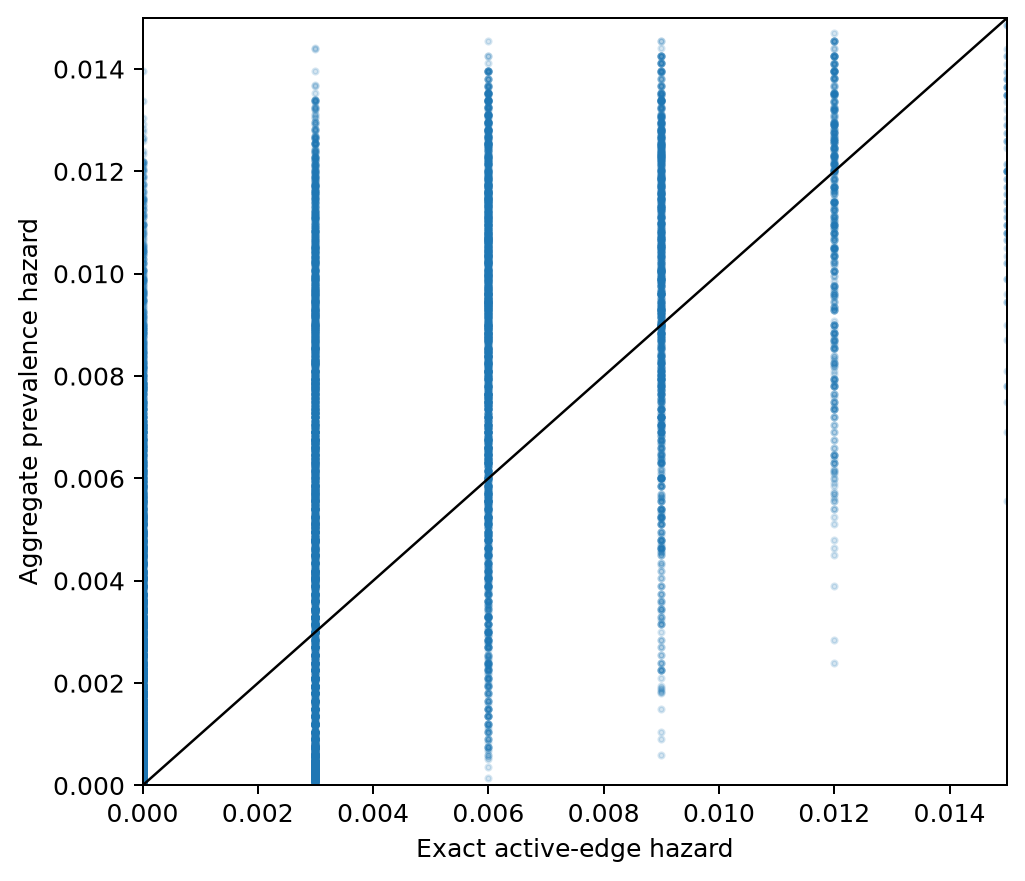
\includegraphics[width=.62\linewidth]{figures/01_exact_vs_aggregate.png}\caption{Exact and aggregate hazards evaluated on common Full Micro states. Points are a visualization subsample; inference is replication-level.}\end{figure}
\begin{figure}[H]\centering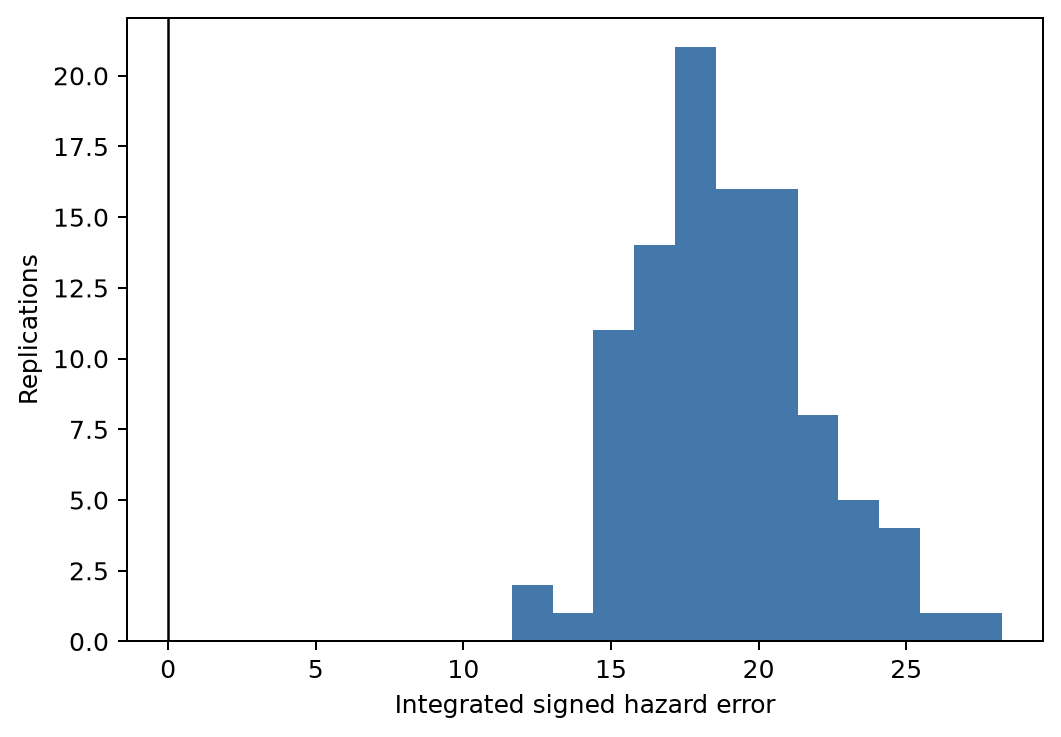
\includegraphics[width=.49\linewidth]{figures/02_signed_error_distribution.png}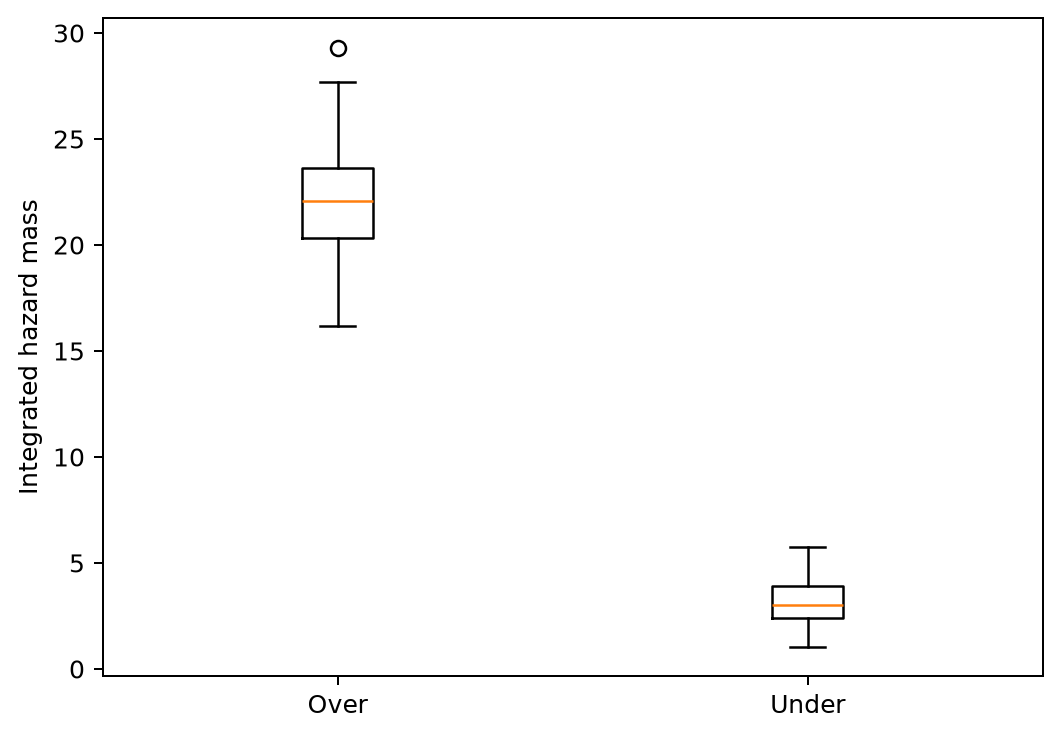
\includegraphics[width=.49\linewidth]{figures/03_over_under_mass.png}\caption{Replication distributions of integrated signed error and its over/under components.}\end{figure}
\begin{figure}[H]\centering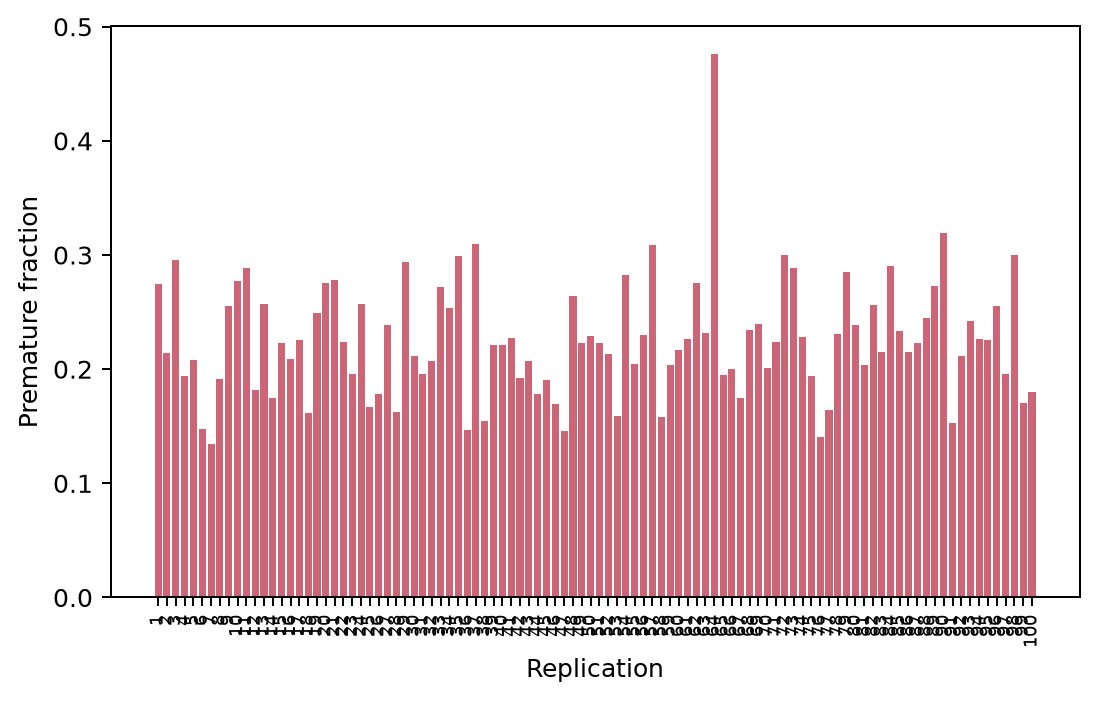
\includegraphics[width=.62\linewidth]{figures/04_premature_fraction.png}\caption{Fraction of aggregate cumulative hazard accumulated when exact inter-community transmission is impossible.}\end{figure}
\begin{figure}[H]\centering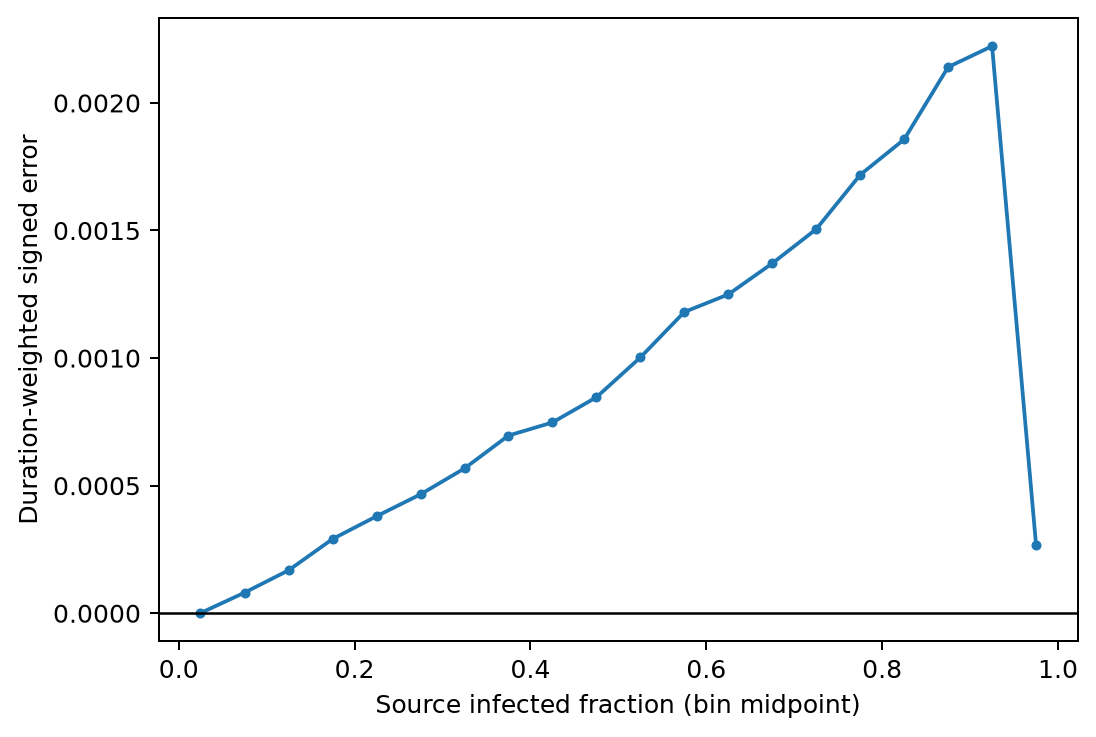
\includegraphics[width=.49\linewidth]{figures/05_error_vs_source_fraction.png}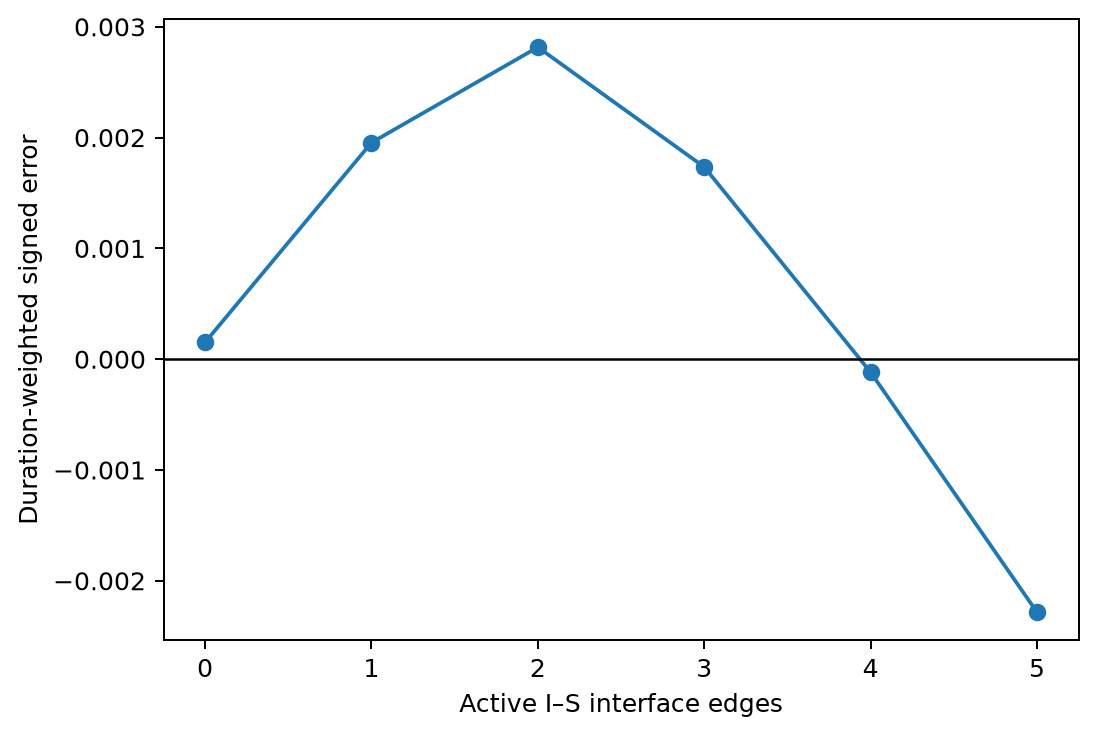
\includegraphics[width=.49\linewidth]{figures/06_error_vs_active_edges.png}\caption{Descriptive event-level stratification. Intervals are dependent and are not treated as independent observations.}\end{figure}
\begin{figure}[H]\centering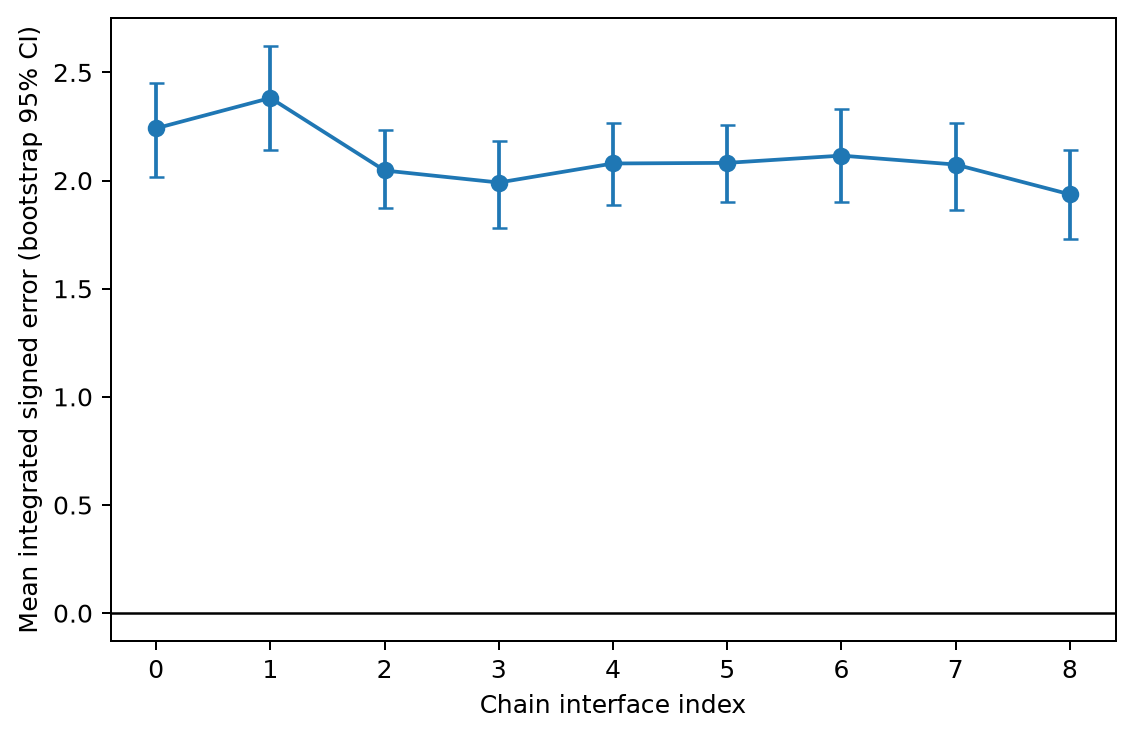
\includegraphics[width=.49\linewidth]{figures/07_layer_integrated_error.png}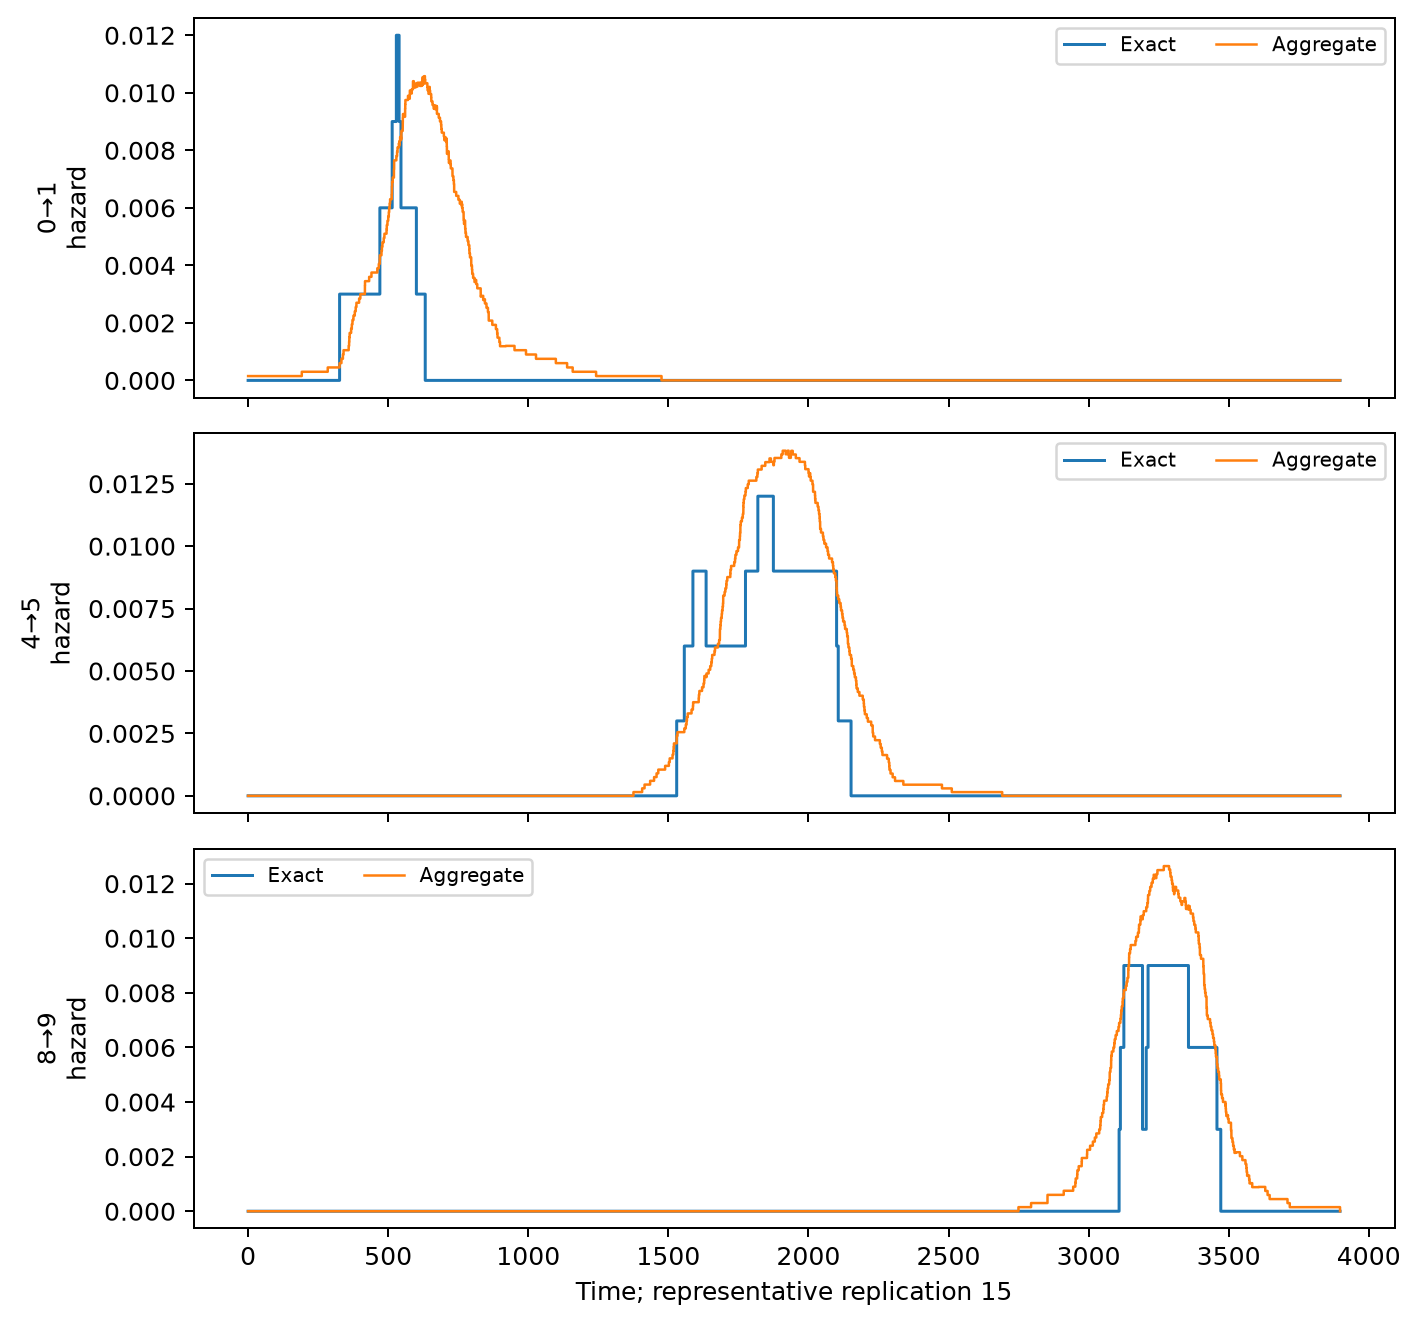
\includegraphics[width=.49\linewidth]{figures/08_representative_time_series.png}\caption{Layer-wise integrated error and representative common-state time series. Uncertainty claims use replication summaries.}\end{figure}

\section{Scientific interpretation}
The signed mass must be interpreted together with absolute, over-, under-, and cumulative premature components: cancellation can make signed error small even when local discrepancies are large. The reported final estimates characterize pure formula-level rate-abstraction error for this baseline. Both over- and under-hazard mass are present, although the replication-level mean over-hazard component is larger for this baseline. This does not establish that aggregate hazards universally overestimate exact hazards.

Across replications, mean cumulative exact and aggregate hazards were 27.131 and 46.078; mean signed and absolute discrepancy masses were 18.947 and 25.154. Mean over-hazard mass (22.05) exceeded mean under-hazard mass (3.1035), but the nonzero under component confirms state-dependent sign changes. A mean 22.537\% of aggregate cumulative hazard accumulated in states with zero exact active-edge hazard (95\% bootstrap interval 21.56--23.611\%). The phase-stratified mean premature fractions were 79.201\% early, 30.165\% middle, and 20.022\% late. These phase values describe where formula mismatch occurs on the replayed trajectories; they are not independent event-level estimates.

\section{What this experiment explains---and does not explain}
It explains discrepancies between two hazard formulas on common Full Micro states. It cannot explain import-placement error, production synchronization error, full endogenous trajectory error, event-time bias by signed error alone, or robustness to other topologies or $\gamma>0$.

\section{Limitations}
This final analysis has 100 replications. Network edges were regenerated rather than archived by Experiment 01. Event-level correlations are descriptive because intervals within a replication are dependent. The phase thresholds are mechanistic fixed bands, not data-selected changepoints. Generalization remains limited to the chain topology and $\gamma=0$ baseline.

\section{Recommended next experiments}
Experiment 03 is the Production vs Event-Driven Synchronization Audit, intended to explain the difference between approximately 7.5\% error for event-driven aggregate/uniform Experiment 01 and approximately 42.6\% in the production sparse benchmark. Experiment 04 is the Gateway-Distance Experiment with near/medium/far gateway placement at fixed $n,m,d,k,\beta$, and community count. Experiment 04 was not run here.

\section{Exact reproduction commands}
\begin{verbatim}
.venv/bin/python -m unittest tests.test_experiment_02_state_replay_hazard_audit
.venv/bin/python extrascripts/run_experiment_02_state_replay_hazard_audit.py --stage smoke --resume
.venv/bin/python extrascripts/run_experiment_02_state_replay_hazard_audit.py --stage validation --resume
.venv/bin/python extrascripts/analyze_experiment_02_state_replay_hazard_audit.py --stage validation
# Only after explicit approval:
.venv/bin/python extrascripts/run_experiment_02_state_replay_hazard_audit.py --stage final --audit-approved --resume
\end{verbatim}
\end{document}
